\documentclass[french,a4paper,10pt]{article}
% uncomment the following lines after copying the template
\input{../../common/common_header.tex}
\input{../../common/macros/math.tex}
\input{../../common/macros/theorems.tex}
% % ============================================================================== 
% GENERAL MATH SHORTCUTS
% ==============================================================================

\newcommand{\abs}[1]{\left\lvert#1\right\rvert}  % Absolute value with scalable bars
\counterwithout{tdcounter}{section} 
\usetikzlibrary{shapes,arrows,positioning,calc,fit,backgrounds,angles,quotes}
% \newcommand{\becomes}{\begin{center}\(\downarrow\)\end{center}}


% ============================================================================== 
% JULIA CODE STUFF
% ==============================================================================


\usepackage{floatrow}
\usepackage{caption}
\usepackage{cases}


\usepackage{listings}
\usepackage{xcolor}

% ----- Julia language definition -----
\lstdefinelanguage{julia}{
    keywords={function, end, if, else, elseif, while, for, in, return, break, continue, struct, 
    mutable, using, import, module, export, const, let, global, local, abstract, typealias, 
    sin, atan, true, add},
    sensitive=true,
    comment=[l]{\#},
    morestring=[b]", % chktex 18
}
\definecolor{codebg}{RGB}{245,245,245}   % very light gray
\definecolor{codeborder}{RGB}{220,220,220} 
\definecolor{keywordcolor}{RGB}{0,0,150}
\definecolor{commentcolor}{RGB}{120,120,120}
\lstdefinestyle{julia-style}{
    language=julia, % new language
    basicstyle=\ttfamily\small,
    keywordstyle=\color{keywordcolor},
    commentstyle=\color{commentcolor},
    stringstyle=\color{verdant},
    backgroundcolor=\color{codebg},
    frame=single,
    framerule=0.5pt,
    rulecolor=\color{codeborder},
    tabsize=2,
    columns=fullflexible,
    keepspaces=true,
    showstringspaces=false,
}
% convenience macro
\newcommand{\juliaFile}[1]{\lstinputlisting[style=julia-style]{#1}}

% custom bash environment with same style as julia
\lstdefinelanguage{bash}{
    keywords={sudo, apt-get, install, update, upgrade, cd, ls, mkdir, rm, rmdir, touch, nano, vim, cat, echo, pwd, cp, mv},
    sensitive=true,
    comment=[l]{\#},
    morestring=[b]", % chktex 18
}
\lstdefinestyle{bash-style}{
    language=bash,
    basicstyle=\ttfamily\small,
    keywordstyle=\color{keywordcolor},
    commentstyle=\color{commentcolor},
    backgroundcolor=\color{codebg},
    frame=single,
    framerule=0.5pt,
    rulecolor=\color{codeborder},
    tabsize=2,
    columns=fullflexible,
    keepspaces=true,
    showstringspaces=false,
}
% convenience macro
\newcommand{\bashFile}[1]{\lstinputlisting[style=bash-style]{#1}}

% ============================================================================== 
% ALGORITHM STUFF
% ==============================================================================
\usepackage[noend]{algpseudocode}
\DeclareCaptionType{algorithm}[Algorithme][Liste des Algorithmes]
\captionsetup[algorithm]{justification=raggedright,singlelinecheck=false}

\newcommand*\Let[2]{\State #1 $\gets$ #2} % chktex 1
\algrenewcommand\alglinenumber[1]{
    {\sf\footnotesize\addfontfeatures{Colour=888888,Numbers=Monospaced}#1}}
\algrenewcommand\algorithmicrequire{\textbf{Input:}}
\algrenewcommand\algorithmicensure{\textbf{Question:}}

\usepackage[a4paper,hmargin=30mm,vmargin=30mm]{geometry}

\title{\color{astral} \sffamily \bfseries Course Name --- TDs}
\author{Ivan Lejeune}
\date{\today}

\toggletrue{showsolutions} % Allows showing/hiding solutions
% uncomment the following line to hide solutions
% \togglefalse{showsolutions}

\begin{document}
    \maketitle
    \tableofcontents

    \newpage
    \section*{TD1 --- Résolution de problèmes --- Modélisation et recherche aveugle}\label{sec:TD1}
    \addcontentsline{toc}{section}{\nameref{sec:TD1}}
    \setcounter{section}{1}
    \setcounter{tdcounter}{0}
    \section{Structures mathématiques}\label{sec:s_1}
% ----- Consignes exo 1 ----- %
\begin{td-exo}[Représentation et facettes]\,\\ % 1 
	Soit \(P_{\varepsilon}\) le polyèdre défini par les inégalités linéaires suivantes:
    \begin{equation*}
        (P_{\varepsilon}) = 
        \begin{cases}
            x_2 \leq 3\\
            \varepsilon x_1 + (2 -\varepsilon) x_2 \leq 4\\
            x_i \geq 0,\forall i \in \{1, 2\}
        \end{cases}
    \end{equation*}
    \begin{enumerate}
        \item Illustrer le polyèdre \(P_\varepsilon\) et les inégalités dans le plan pour \(\varepsilon = 1\) et \(\varepsilon = -1\).

        \item Soient \(\varepsilon = 3\) et le polyèdre entier \(P_I = \conv(P_3 \cap \bb Z^2)\).
        Dessiner \(P_I\) et donner une représentation (extérieure) minimale de \(P_I\).
    \end{enumerate}
\end{td-exo}

% ----- Solutions exo 1 ----- %
\iftoggle{showsolutions}{ 
	\begin{td-sol}[]\ % 1
		\begin{enumerate}
            \item Pour \(\varepsilon = -1\), le problème \(P_\varepsilon\) devient le suivant:
            \begin{equation*}
                P_\varepsilon = P_{-1} = 
                \begin{cases}
                    x_2 \leq 3\\
                    - x_1 + 3 x_2 \leq 4\\
                    x_i \geq 0,\forall i \in \{1, 2\}
                \end{cases}
            \end{equation*}
            On peut représenter ce problème dans le plan comme suit:

            \vspace{2mm}
\ffigbox[\FBwidth]{%
\caption{\centering Représentation du problème \(P_\varepsilon\) dans \(\bb R^2\) pour \(\varepsilon = -1\)}\label{fig:dm1_ex01_f1}
}{
    \fbox{
        \begin{tikzpicture}
            \begin{axis}[
                % axis lines=middle,
                xlabel={\(x_1\)},
                ylabel={\(x_2\)},
                xmin=0, xmax=6.5,
                ymin=0, ymax=4,
                grid=both,
                axis equal image, % <-- orthonormal grid
                width=10cm,
                height=7cm,
                legend pos=outer north east, % <-- legend outside
                legend cell align=left,
                legend image post style={fill opacity=0.45},
                legend style={fill=pagebg, draw=pagetext}
            ]

            % ----- Constraint lines -----

            % x2 = 3  -> x2 = 3
            \addplot[domain=0:6.5, very thick, color=blue] {3};
            \addlegendentry{\(x_2 = 3\)}

            % -x1 + 3x2 = 4 -> x2 = (4 + x1)/3
            \addplot[domain=0:6.5, very thick, color=orange] {4/3 + x/3};
            \addlegendentry{\(-x_1 + 3x_2 = 4\)}

            % % x2 = 2
            % \addplot[domain=0:3, very thick, color=green!60!black] {2};
            % \addlegendentry{\(x_2 = 2\)}

            % ----- Feasible region -----
            \addplot[
                fill=cyan!30,
                opacity=0.45,
                draw=none,
                area legend
            ] coordinates {
                (0, 0)
                (0, 4/3)
                (5, 3)
                (6.5, 3)
                (6.5, 0)
            };
            \addlegendentry{Région réalisable}

            % % ----- Optimal real solution -----
            % \addplot[
            %     only marks,
            %     mark=*,
            %     mark size=2.5pt,
            %     color=red!80!black
            % ] coordinates {(0.75,0.25)};
            % \addlegendentry{Solution réelle}

            % % ----- Optimal integer solution -----
            % \addplot[
            %     only marks,
            %     mark=square*,
            %     mark size=2.5pt,
            %     color=purple
            % ] coordinates {(1,0)};
            % \addlegendentry{Solution entière}
            
            % % Draw the objective level line
            % \addplot[dashed, thick, yellow, domain=0:2] {3*x - 2};
            % \addlegendentry{Ligne de niveau \(z=2\)}

            % Draw the direction of decrease (vector)
            % \draw[->, thick, red!70!black] 
            %     (axis cs:0.75,0.25) -- (axis cs:0.75-0.6,0.25+0.2) 
            %     node[above left] {$(-3,1)$};
            \end{axis}
        \end{tikzpicture}
    }
}

            Quelques remarques par rapport à la figure:
            \begin{itemize}
                \item Tout d'abord on peut remarquer que l'ensemble des points dans le polyèdre est non borné en \(x_1\).
                \item Les points extrêmes de ce polyèdre sont:
                \begin{equation*}
                    (0, 0), (0, 4/3), (5, 3), (6.5, 3), (6.5, 0)
                \end{equation*}
            \end{itemize}

            Regardons maintenant le cas \(\varepsilon = 1\). Le problème \(P_\varepsilon\) devient le suivant:
            \begin{equation*}
                P_\varepsilon = P_{1} = 
                \begin{cases}
                    x_2 \leq 3\\
                    x_1 + x_2 \leq 4\\
                    x_i \geq 0,\forall i \in \{1, 2\}
                \end{cases}
            \end{equation*}
            On peut représenter ce problème dans le plan comme suit:

            \vspace{2mm}
\ffigbox[\FBwidth]{%
\caption{\centering Représentation du problème \(P_\varepsilon\) dans \(\bb R^2\) pour \(\varepsilon = 1\)}\label{fig:dm1_ex01_f2}
}{
    \fbox{
        \begin{tikzpicture}
            \begin{axis}[
                xlabel={\(x_1\)},
                ylabel={\(x_2\)},
                xmin=0, xmax=5,
                ymin=0, ymax=5,
                grid=both,
                axis equal image,
                width=10cm,
                height=7cm,
                legend pos=outer north east,
                legend cell align=left,
                legend image post style={fill opacity=0.45},
                legend style={fill=pagebg, draw=pagetext}
            ]

            % ----- Constraint lines -----

            % x2 = 3  -> x2 = 3
            \addplot[domain=0:5, very thick, color=blue] {3};
            \addlegendentry{\(x_2 = 3\)}

            % x1 + x2 = 4 -> x2 = 4 - x1
            \addplot[domain=0:5, very thick, color=orange] {4 - x};
            \addlegendentry{\(x_1 + x_2 = 4\)}

            % ----- Feasible region -----
            \addplot[
                fill=cyan!30,
                opacity=0.45,
                draw=none,
                area legend
            ] coordinates {
                (0, 0)
                (0, 3)
                (1, 3)
                (4, 0)
            };
            \addlegendentry{Région réalisable}
            \end{axis}
        \end{tikzpicture}
    }
}

            Quelques remarques par rapport à la figure:
            \begin{itemize}
                \item Tout d'abord on peut remarquer que l'ensemble des points dans le polyèdre est complètement borné cette fois-ci.
                Contrairement au cas \(\varepsilon = -1\), on ne peut pas choisir n'importe quelle valeur pour \(x_1\).
                \item Les points extrêmes de ce polyèdre sont:
                \begin{equation*}
                    (0, 0), (0, 3), (1, 3), (4, 0)
                \end{equation*}
                \item Ces deux problèmes, même s'ils viennent tous deux de \(P_\varepsilon\) ont des représentations dans l'espace bien différentes, cela est notamment dû à l'impact qu'a le choix de \(\varepsilon\) sur le signe des variables \(x_1\) et \(x_2\) dans la seconde contrainte. C'est ce qui décide \og{}l'angle de la pente\fg{} de cette contrainte et qui permet donc de borner ou non le polyèdre.
            \end{itemize}

            \item On fixe désormais \(\varepsilon = 3\). On commence par représenter le problème \(P_3\) dans l'espace comme suit:

            \vspace{2mm}
\ffigbox[\FBwidth]{%
\caption{\centering Représentation du problème \(P_\varepsilon\) dans \(\bb R^2\) pour \(\varepsilon = 3\)}\label{fig:dm1_ex01_f3}
}{
    \fbox{
        \begin{tikzpicture}
            \begin{axis}[
                xlabel={\(x_1\)},
                ylabel={\(x_2\)},
                xmin=0, xmax=3,
                ymin=0, ymax=4,
                grid=both,
                axis equal image,
                width=10cm,
                height=7cm,
                legend pos=outer north east,
                legend cell align=left,
                legend image post style={fill opacity=0.45},
                legend style={fill=pagebg, draw=pagetext}
            ]

            % ----- Constraint lines -----

            % x2 = 3  -> x2 = 3
            \addplot[domain=0:3, very thick, color=blue] {3};
            \addlegendentry{\(x_2 = 3\)}

            % 3x1 - x2 = 4 -> x2 = 3x1 - 4
            \addplot[domain=0:3, very thick, color=orange] {3*x - 4};
            \addlegendentry{\(3x_1 - x_2 = 4\)}

            % ----- Feasible region -----
            \addplot[
                fill=cyan!30,
                opacity=0.45,
                draw=none,
                area legend
            ] coordinates {
                (0, 0)
                (0, 3)
                (7/3, 3)
                (4/3, 0)
            };
            \addlegendentry{Région réalisable}
            \end{axis}
        \end{tikzpicture}
    }
}

            Ensuite, on veut contraindre cet ensemble de points pour se retrouver uniquement avec des valeurs entières. 
            Cela donne le graphe suivant:

            \vspace{2mm}
\ffigbox[\FBwidth]{%
\caption{\centering Représentation de l'ensemble de points \(P_3 \cap \bb Z^2\) dans \(\bb R^2\)}\label{fig:dm1_ex01_f4}
}{
    \fbox{
        \begin{tikzpicture}
            \begin{axis}[
                xlabel={\(x_1\)},
                ylabel={\(x_2\)},
                xmin=0, xmax=3,
                ymin=0, ymax=4,
                grid=both,
                axis equal image,
                width=10cm,
                height=7cm,
                legend pos=outer north east,
                legend cell align=left,
                legend image post style={fill opacity=0.45},
                legend style={fill=pagebg, draw=pagetext}
            ]

            % ----- Constraint lines -----

            % x2 = 3  -> x2 = 3
            \addplot[domain=0:3, very thick, color=blue] {3};
            \addlegendentry{\(x_2 = 3\)}

            % 3x1 - x2 = 4 -> x2 = 3x1 - 4
            \addplot[domain=0:3, very thick, color=orange] {3*x - 4};
            \addlegendentry{\(3x_1 - x_2 = 4\)}

            % ----- Feasible region -----
            \addplot[
                fill=cyan!30,
                opacity=0.45,
                draw=none,
                area legend
            ] coordinates {
                (0, 0)
                (0, 3)
                (7/3, 3)
                (4/3, 0)
            };
            \addlegendentry{Région réalisable de \(P_3\)}

            % ----- Integer points inside the feasible region -----
            \foreach \x in {0,1}{
                \foreach \y in {0,1,2,3}{
                    \addplot[
                        only marks,
                        mark=*,
                        mark size=2.2pt,
                        color=green!70
                    ] coordinates {(\x,\y)};
                }
            }
            \addplot[
                only marks,
                mark=*,
                mark size=2.2pt,
                color=green!70
            ] coordinates {(2,2)};
            \addplot[
                only marks,
                mark=*,
                mark size=2.2pt,
                color=green!70
            ] coordinates {(2,3)};
            \addlegendentry{Ensemble de points dans \(P_3 \cap \bb Z^2\)}
            \end{axis}
        \end{tikzpicture}
    }
}

            On veut maintenant trouver l'enveloppe convexe de cet ensemble de points ce qui donne le graphe suivant:

            \input{../assets/tikz/dm1_ex01_f5.tex}

            Enfin, on peut nettoyer un peu la figure pour voir plus clairement l'enveloppe convexe:

            \vspace{2mm}
\ffigbox[\FBwidth]{%
\caption{\centering Représentation de l'enveloppe convexe de \(P_3 \cap \bb Z^2\) dans \(\bb R^2\) nettoyée}\label{fig:dm1_ex01_f6}
}{
    \fbox{
        \begin{tikzpicture}
            \begin{axis}[
                % axis lines=middle,
                xlabel={\(x_1\)},
                ylabel={\(x_2\)},
                xmin=0, xmax=3,
                ymin=0, ymax=4,
                grid=both,
                axis equal image, % <-- orthonormal grid
                width=10cm,
                height=7cm,
                legend pos=outer north east, % <-- legend outside
                legend cell align=left,
                legend image post style={fill opacity=0.45},
                legend style={fill=pagebg, draw=pagetext}
            ]

            % ----- Constraint lines -----

            % % x2 = 3  -> x2 = 3
            % \addplot[domain=0:3, very thick, color=blue] {3};
            % \addlegendentry{\(x_2 = 3\)}

            % % 3x1 - x2 = 4 -> x2 = 3x1 - 4
            % \addplot[domain=0:3, very thick, color=orange] {3*x - 4};
            % \addlegendentry{\(3x_1 - x_2 = 4\)}

            % % x2 = 2
            % \addplot[domain=0:3, very thick, color=green!60!black] {2};
            % \addlegendentry{\(x_2 = 2\)}

            % % ----- Feasible region -----
            % \addplot[
            %     fill=cyan!30,
            %     opacity=0.45,
            %     draw=none,
            %     area legend
            % ] coordinates {
            %     (0, 0)
            %     (0, 3)
            %     (7/3, 3)
            %     (4/3, 0)
            % };
            % \addlegendentry{Région réalisable de \(P_3\)}

            % ----- Integer points inside the feasible region -----
            \foreach \x in {0,1}{
                \foreach \y in {0,1,2,3}{
                    \addplot[
                        only marks,
                        mark=*,
                        mark size=2.2pt,
                        color=green!70,
                        forget plot
                    ] coordinates {(\x,\y)};
                }
            }
            \addplot[
                only marks,
                mark=*,
                mark size=2.2pt,
                color=green!70,
                forget plot
            ] coordinates {(2,2)};
            \addplot[
                only marks,
                mark=*,
                mark size=2.2pt,
                color=green!70
            ] coordinates {(2,3)};
            \addlegendentry{Ensemble de points dans \(P_3 \cap \bb Z^2\)}
            
            % ----- Smaller Feasible region -----
            \addplot[
                fill=red!30,
                opacity=0.45,
                draw=none,
                area legend
            ] coordinates {
                (0, 0)
                (0, 3)
                (2, 3)
                (2, 2)
                (1, 0)
            };
            \addlegendentry{Enveloppe convexe de \(P_3 \cap \bb Z^2\)}

            % % ----- Optimal real solution -----
            % \addplot[
            %     only marks,
            %     mark=*,
            %     mark size=2.5pt,
            %     color=red!80!black
            % ] coordinates {(0.75,0.25)};
            % \addlegendentry{Solution réelle}

            % % ----- Optimal integer solution -----
            % \addplot[
            %     only marks,
            %     mark=square*,
            %     mark size=2.5pt,
            %     color=purple
            % ] coordinates {(1,0)};
            % \addlegendentry{Solution entière}
            
            % % Draw the objective level line
            % \addplot[dashed, thick, yellow, domain=0:2] {3*x - 2};
            % \addlegendentry{Ligne de niveau \(z=2\)}

            % Draw the direction of decrease (vector)
            % \draw[->, thick, red!70!black] 
            %     (axis cs:0.75,0.25) -- (axis cs:0.75-0.6,0.25+0.2) 
            %     node[above left] {$(-3,1)$};
            \end{axis}
        \end{tikzpicture}
    }
}

            On voit alors que ce polyèdre \(P_I\) est clairement défini par les trois contraintes suivantes:
            \begin{equation*}
                (P_I) = 
                \begin{cases}
                    x_2 \leq 3\\
                    x_1 \leq 2\\
                    2x_1 - x_2 \leq 2\\
                    x_i \geq 0,\ \forall i \in \{1, 2\}
                \end{cases}
            \end{equation*}
            ce qui donne le graphe suivant:

            \vspace{2mm}
\ffigbox[\FBwidth]{%
\caption{\centering Représentation du polyèdre \(P_I\) dans \(\bb R^2\)}\label{fig:dm1_ex01_f7}
}{
    \fbox{
        \begin{tikzpicture}
            \begin{axis}[
                xlabel={\(x_1\)},
                ylabel={\(x_2\)},
                xmin=0, xmax=3,
                ymin=0, ymax=4,
                grid=both,
                axis equal image,
                width=10cm,
                height=7cm,
                legend pos=outer north east,
                legend cell align=left,
                legend image post style={fill opacity=0.45},
                legend style={fill=pagebg, draw=pagetext}
            ]

            % ----- Constraint lines -----

            % x2 = 3  -> x2 = 3
            \addplot[domain=0:3, very thick, color=blue] {3};
            \addlegendentry{\(x_2 = 3\)}
            
            % x1 = 2
            \addplot[
                very thick,
                color=orange
            ] coordinates {(2,0) (2,4)};
            \addlegendentry{\(x_1 = 2\)}

            % 2x1 - x2 = 2 -> x2 = 2x1 - 2
            \addplot[domain=0:3, very thick, color=green!60!black] {2*x - 2};
            \addlegendentry{\(2x_1 - x_2 = 2\)}
            
            % ----- Smaller Feasible region -----
            \addplot[
                fill=red!30,
                opacity=0.45,
                draw=none,
                area legend
            ] coordinates {
                (0, 0)
                (0, 3)
                (2, 3)
                (2, 2)
                (1, 0)
            };
            \addlegendentry{Enveloppe convexe de \(P_I\)}
            \end{axis}
        \end{tikzpicture}
    }
}

            Quelques remarques sur \(P_I\):
            \begin{itemize}
                \item Comme pour le cas \(\varepsilon = 1\), l'ensemble des points du polyèdre est borné.
                Plus fort que ca, les différents points du polyèdre sont bornés par des points entiers.
                \item Les points extrêmes de ce polyèdre sont:
                \begin{equation*}
                    (0, 0), (0, 3), (2, 3), (2, 2), (1, 0)
                \end{equation*}
                \item Tous les points extrêmes de \(P_I\) sont entiers.
                \item Le polyèdre \(P_I\) est entièrement défini par 3 inégalités.
            \end{itemize}
        \end{enumerate}
	\end{td-sol}
}{}
% ----- Consignes exo 2 ----- %
\begin{td-exo}[Autour de \textsc{Satisfaisabilité}]\, % 2 
	\vspace{-6mm}
\begin{algorithm}[H]
    \caption{\textsc{Non Egal Satisfaisabilité} (NAESAT)}
    \begin{algorithmic}
        \Require{Une formule conjonctive \(\varphi\) sur \(n\) variables et \(m\) clauses}
        \Ensure{Existe-t-il une affectation de valeurs de vérité aux variables qui satisfasse \(\varphi\) tel que chaque clause a un littéral vrai et un littéral faux?}
    \end{algorithmic}
\end{algorithm}
	
	Montrer que \textsc{Non Egal Satisfaisabilité} est \(\mathcal{NP}\)-\textit{complet}. 
	La preuve se fera à partir de \textsc{Satisfaisabilité}.
\end{td-exo}

% ----- Solutions exo 2 ----- %
\iftoggle{showsolutions}{ 
	\begin{td-sol}[]\ % 2
		Le problème de \textsc{Non Egal Satisfaisabilité} est dans \(\mathcal{NP}\) car on peut vérifier en temps polynomial si deux formules booléennes sont non équivalentes. 
		Pour montrer qu'il est \(\mathcal{NP}\)-complet, on effectue une réduction à partir du problème de \textsc{Satisfaisabilité}. 
		On montre que si on pouvait résoudre \textsc{Non Egal Satisfaisabilité} en temps polynomial, alors on pourrait résoudre \textsc{Satisfaisabilité} en temps polynomial, ce qui contredit l'hypothèse que \(\mathcal{P} \neq \mathcal{NP}\). 
		Par conséquent, \textsc{Non Egal Satisfaisabilité} est \(\mathcal{NP}\)-complet.

		Soit \(\varphi\) une formule conjonctive de \(3\)-\textsc{SAT}. 
		On construit une formule \(\psi\) pour le problème de \textsc{Non Egal Satisfaisabilité} de la manière suivante:
		\begin{equation*}
			\psi_i = \varphi_i \land (x_1 \lor \ldots \lor x_n) \land (\lnot x_1 \lor \ldots \lor \lnot x_n), \quad \forall i \in \{1, \ldots, m\}
		\end{equation*}

		Ensuite, on pose \(\psi = \bigwedge_{i=1}^m \psi_i\).
		
		Si \(\varphi\) est satisfaisable, alors il existe une affectation de valeurs de vérité aux variables qui satisfait \(\varphi\). 
		Cette même affectation satisfait également \(\psi\) car les clauses supplémentaires garantissent que chaque clause de \(\psi\) a un littéral vrai et un littéral faux.
		
		Inversement, si \(\psi\) est satisfaisable, alors il existe une affectation de valeurs de vérité aux variables qui satisfait \(\psi\). 
		Cette affectation doit également satisfaire \(\varphi\) (car si elle satisfait chaque clause de \(\psi\)), alors elle satisfait également chaque clause de \(\varphi\). 
		
		Par conséquent, \(\varphi\) est satisfaisable si et seulement si \(\psi\) est satisfaisable, ce qui montre que le problème de \textsc{Non Egal Satisfaisabilité} est \(\mathcal{NP}\)-complet (car il est au moins aussi dur que \textsc{Satisfaisabilité}, qui est lui-même \(\mathcal{NP}\)-complet).
	\end{td-sol}
}{}

% ----- Consignes exo 3 ----- %
\begin{td-exo}[Quelques preuves de NP-complétude pour \textsc{Steiner tree}]\,\\ % 3 
	\input{../assets/tikz/td1_ex03_1.tex}
	\input{../assets/tikz/td1_ex03_2.tex}
	\input{../assets/tikz/td1_ex03_3.tex}

	\begin{enumerate}
		\item Montrer que \textsc{Steiner Tree} est NP-complet.
		Procéder à une réduction à partir de \textsc{Exact Cover by 3-Sets}.

		\item Montrer que \textsc{Steiner Tree} est NP-complet par une réduction à partir de \textsc{Vertex Cover}.
	\end{enumerate}
\end{td-exo}

% ----- Solutions exo 3 ----- %
\iftoggle{showsolutions}{ 
	\begin{td-sol}[]\ % 3
		
	\end{td-sol}
}{}


    \newpage
    \section*{TD2 --- Recherche de solution optimale}\label{sec:TD2}
    \addcontentsline{toc}{section}{\nameref{sec:TD2}}
    \setcounter{section}{2}
    \setcounter{tdcounter}{0}
    % ----- Consignes exo 1 ----- %
\begin{td-exo}[Euh \dots]\,\\ % 1 
	Que vaut \(\alpha(L(G))\)?
\end{td-exo}

% ----- Solutions exo 1 ----- %
\iftoggle{showsolutions}{
	\begin{td-sol}[]\,\\ %
		On a
		\begin{equation*}
			\alpha(L(G)) = \mu(G)
		\end{equation*}
	\end{td-sol}
}{}


% ----- Consignes exo 2 ----- %
\begin{td-exo}[Couplage maximum Vs couplage maximal]\,\\ % 2 
	Soient \(G\) un graphe, \(M\) un couplage maximal de 
	\(G\) et \(M^\ast\) un couplage maximum de \(G\).
	Montrer que \(|M| \leq |M^\ast| \leq 2|M|\).
\end{td-exo}

% ----- Solutions exo 2 ----- %
\iftoggle{showsolutions}{
	\begin{td-sol}[]\,\\ %
		On peut considérer le stable \(S\) tel que 
		\(S\cup M = G\).
	\end{td-sol}
}{}


% ----- Consignes exo 3 ----- %
\begin{td-exo}[Couplage dans les graphes sans triangle]\,\\ % 3 
	Un graphe est dit sans triangle si il ne contient pas 
	de cycle de longueur 3 comme sous-graphe. Si \(G\) 
	est sans triangle, montrer que
	\begin{equation*}
		\chi(\ol G) + \mu(G) = n
	\end{equation*}
\end{td-exo}

% ----- Solutions exo 3 ----- %
\iftoggle{showsolutions}{
	\begin{td-sol}[]\,\\ %
		A remplir %TODO solve exercise 3
	\end{td-sol}
}{}


% ----- Consignes exo 4 ----- %
\begin{td-exo}[Jeu de Slither]\,\\ % 4 
	Le \emph{jeu de Slither} se joue sur un graphe connexe, noté \(G\).
	Chaque joueur choisit à son tour un sommet \(v_i\) non
	précédemment choisi. La suite \(v_0,v_1,\ldots\) doit former un chemin,
	c'est-à-dire que tout pour tout \(i=1, 2,\ldots\),  \(v_i\) doit être
	choisi comme adjacent à \(v_{i-1}\). Le joueur qui ne peut plus 
	jouer a perdu.

	Montrer que si \(G\) admet un couplage parfait alors le second joueur
	a une stratégie gagnante. Montrer que si \(G\) n'admet pas un 
	couplage parfait alors le premier joueur a une stratégie gagnante
\end{td-exo}

% ----- Solutions exo 4 ----- %
\iftoggle{showsolutions}{
	\begin{td-sol}[]\,\\ %
		A remplir %TODO solve exercise 4
	\end{td-sol}
}{}


% ----- Consignes exo 5 ----- %
\begin{td-exo}[Tous d'un coup]\,\label{ex:td2ex5}\\ % 5 
	Soit \(G = (X\cup Y, E)\) un graphe biparti de bipartition \((X, Y)\)
	avec \(\Delta(G) \geq 1\).
	\begin{enumerate}
		\item Montrer que \(G\) admet un couplage couvrant tous les sommets de \(X\) de degré \(\Delta(G)\).
		\item Montrer que \(G\) admet un couplage couvrant tous les sommets de \(G\) de degré \(\Delta(G)\).
		\item En déduire qu'il est possible de partitionner les arêtes de \(G\) en \(\Delta(G)\) couplages.
	\end{enumerate}
\end{td-exo}

% ----- Solutions exo 5 ----- %
\iftoggle{showsolutions}{
	\begin{td-sol}[]\, %
		\begin{enumerate}
			\item On note \(k = \Delta(G)\). Soit \(S\subseteq X_\Delta\).
			On note \(Z = N_G(S)\). On va compter \(e\) le nombre d'aretes
			entre \(S\) et \(Z\):
			\begin{equation*}
				e = \sum_{s\in S} \deg(s) = k\cdot|S|
			\end{equation*}
			Par ailleurs, comme toute arete comptée est incidente à
			un sommet \(z\), on a:
			\begin{equation*}
				e \leq \sum_{z\in Z} \deg(z) = k\cdot|Z| 
			\end{equation*}
			Donc \(k\cdot|S| \leq k\cdot|Z|\) d'où \(|S| \leq |Z| = |N_G(S)|\).
			Par le théorème de Hall, \(G\) admet un couplage qui sature \(X_\Delta\).

			\item Par la question précédente il existe un couplage \(M_X\) saturant
			\(X_\Delta\). De même, il existe un couplage \(M_Y\) saturant
			\(Y_\Delta\). On va extraire de \(M_X\cup M_Y\) un couplage \(M\)
			saturant \(X_\Delta \cup Y_\Delta\). On construit \(M\) en
			regardant chaque composante connexe de \(M_X \cup M_Y\).

			Soit \(C\) une composante connexe de \((V, M_X \cup M_Y\)) (\(C\)
			est soit un chemin soit un cycle).
			\begin{itemize}
				\item Si \(C\) est un cycle
				% insert graph here
				alors on choisit \(M = M_X\) ou \(M = M_Y\) (les deux conviennent)
				et on continue à saturer les sommets de \(C\)

				\item Si \(C\) est un chemin
				% insert graph here
				on peut supposer que sa première arête est dans \(M_X\).
				% inserer 3 graphs disjonction de cas
				On note \(C = x_1 x_2 \ldots x_k\). On a trois cas:
				\begin{enumerate}
					\item Si \(x_1\in Y_\Delta\), c'est impossible car \(x_1\) doit 
					être incident à une arête de \(M_Y\),
					\item Si \(x_1\in Y \setminus Y_\Delta\), on prend \(M = M_Y\),
					\item Si \(x_1\in X_\Delta\) on prend \(M = M_X\).
				\end{enumerate}
			\end{itemize}
		\end{enumerate}
	\end{td-sol}
}{}


% ----- Consignes exo 6 ----- %
\begin{td-exo}[Famille couvrante de cycles dans les graphes \(2k\)-réguliers]\,\\ % 6 
	Un \(2\)\emph{-factor} d'un graphe \(G\) est un sous-graphe \(2\)-régulier couvrant \(G\).
	Le but de l'exercice est de montrer le résultat suivant dû à J. Petersen (1891): 
	\emph{tout graphe régulier de degré pair admet un \(2\)-factor}.
	Soit \(G\) un graphe régulier de degré pair.
	\begin{enumerate}
		\item A l'aide d'une marche eulérienne de \(G\), montrer que \(G\) admet une orientation 
		\(D\) dans laquelle \(d^+(x) = d^-(x)\) pour tout sommet \(x\) de \(G\).

		\item Le \defemph{biparti d'adjacence} d'un graphe orienté \(D = (V, A)\) est le graphe 
		de sommets \(\left\{x^+, x^-,\ : x\in V(D)\right\}\) et d'arêtes 
		\(\left\{u^+ v^-,\ : uv\in A(D)\right\}\). En étudiant le biparti d'adjacence du graphe orienté
		produit à la question précédente, conclure.
	\end{enumerate}
\end{td-exo}

% ----- Solutions exo 6 ----- %
\iftoggle{showsolutions}{
	\begin{td-sol}[]\,\\ %
		A remplir %TODO solve exercise 6
	\end{td-sol}
}{}


% ----- Consignes exo 7 ----- %
\begin{td-exo}[Convexité]\,\\ % 7 
	% fill
\end{td-exo}

% ----- Solutions exo 7 ----- %
\iftoggle{showsolutions}{
	\begin{td-sol}[]\, %
		\begin{enumerate}
			\item On construit le graphe biparti \(((X, Y), E)\)
			avec \(Y=A\) et \(X = \{1,\ldots,p\}\).
			% insert graph here
			On relie \(a\in A\) à \(i\) si \(a\in A_i\).
			Un SDR correspond à un couplage saturant \(X\).

			C'est exactement le théorème de Hall.

			\item Dans le cas où il y a \(p\)-candidats
			potentiels pour \(p\) ensembles, chaque élément
			sera un représentant.

			\item % insert it all here, both graphs and line
		\end{enumerate}
	\end{td-sol}
}{}


% ----- Consignes exo 8 ----- %
\begin{td-exo}[Subtil SAT]\,\\ % 8 
	% fill
\end{td-exo}

% ----- Solutions exo 8 ----- %
\iftoggle{showsolutions}{
	\begin{td-sol}[]\, %
		\begin{enumerate}
			\item Soit \(F\) une formule \(3\)-\(SAT\). Pour \(i=1\ldots s\) nombre de variables,
			si \(x_i\) apparaît \(l_i\) fois, on crée \(l_i\) variables
			\(x_i^1, \ldots, x_i^{l_i}\) dans \(F\), on remplace
			la \(j\)-eme occurence de \(x_i\) par \(x_i^j\).

			On ajoute les clauses
			\begin{equation*}
				\left(
					\lnot x_i^1 \lor x_i^2
				\right)
				\land
				\left(
					\lnot x_i^2 \lor x_i^3
				\right)
				\land \ldots \land
				\left(
					\lnot x_i^{l_i} \lor x_i^1
				\right).
			\end{equation*}
			Elles sont toutes de taille \(\leq 2\) et maintenant toutes
			les variables \(x_i^j\) ont la même valeur.

			On obtient une formule équivalente à \(F\), où les clauses
			sont de taille \(\leq 3\) et les variables apparaissent 3 fois.

			Comme \(3\)-\(SAT\) est NP-complet, \((\leq 3)\)-\(SAT(\leq 3)\)
			est aussi NP-complet.

			\item On fait le biparti \(G\) Clause-Variable.
			% insert graph here
			Les sommets clauses sont de degré 3 dans \(G\).
			Les sommets variables sont de degré \(\leq 3\).

			Par l'exercice~\ref{ex:td2ex5} il existe un couplage \(M\) saturant les clauses.
			Chaque clause \(C_i\) a sa variable privée \(M\cdot C_i\).
			Pour \(i\in\{1,\ldots,n\}\), on instancie \(M\cdot C_i\) 
			pour satisfaire \(C_i\).

			Ainsi, la formule de départ est toujours satisfaisable.

		\end{enumerate}
	\end{td-sol}
}{}
% ----- Consignes exo 9 ----- %
\begin{td-exo}[Algo de couplace max --- Partie 1]\,\\ % 9 
	Dans le graphe biparti suivant, appliquer l'algo de calcul
	d'un couplage maximum, en sachant que le couplage
	\(\{1b, 2c\}\) a déjà été précalculé.
	
	\input{../assets/tikz/td_2_ex_9.tex}
\end{td-exo}

% ----- Solutions exo 9 ----- %
\iftoggle{showsolutions}{
	\begin{td-sol}[]\,\\ %
		On commence par \(a\) non saturé
		et on fait l'arbre de couplage.
		\begin{itemize}
			\item On trouve \(1, 2\) à partir de \(a\),
			\item puis on trouve \(b, c\) et on barre les chemins reliés,
			\item on trouve \(4\) à partir de \(b\), il est non saturé donc
			\(a1b4\) est augmentant.
			\item On augmente \(|M|\) et on recommence.
		\end{itemize}
		\,
		\begin{itemize}
			\item Je choisis \(e\) non saturé, 
			\item \(5\) est non saturé donc \(e5\) est augmentant.
			\item On augmente \(|M|\) et on recommence.
		\end{itemize}
		
		% Figure 1
\ffigbox[\FBwidth]{
\label{Fig:td2ex9}
}{
    \fbox{
        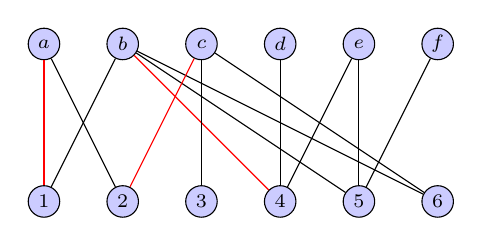
\begin{tikzpicture}[scale=1, every node/.style={circle, draw, fill=blue!20, inner sep=1pt, font=\scriptsize, minimum size=4mm}]
            \node (a) at (0, 2) {\(a\)};
            \node (b) at (1, 2) {\(b\)};
            \node (c) at (2, 2) {\(c\)};
            \node (d) at (3, 2) {\(d\)};
            \node (e) at (4, 2) {\(e\)};
            \node (f) at (5, 2) {\(f\)};

            \node (1) at (0, 0) {\(1\)};
            \node (2) at (1, 0) {\(2\)};
            \node (3) at (2, 0) {\(3\)};
            \node (4) at (3, 0) {\(4\)};
            \node (5) at (4, 0) {\(5\)};
            \node (6) at (5, 0) {\(6\)};

            \draw[red] (a) -- (1);
            \draw (a) -- (2);

            \draw (b) -- (1);
            \draw[red] (b) -- (4);
            \draw (b) -- (5);
            \draw (b) -- (6);
            
            \draw[red] (c) -- (2);
            \draw (c) -- (3);
            \draw (c) -- (6);
            
            \draw (d) -- (4);
            
            \draw (e) -- (4);
            \draw (e) -- (5);
            
            \draw (f) -- (5);
        \end{tikzpicture}
    }
}

		\begin{itemize}
			\item Je choisis \(d\) non saturé,
			\item \(6\) est non saturé donc \(d4b6\) est augmentant.
			\item On augmente \(|M|\) et on recommence.
		\end{itemize}
		
		\input{../assets/tikz/td_2_ex_9_2.tex}

		\begin{itemize}
			\item On calcule un arbre de couplage enraciné en \(3\),
			\item Il est complet, on peut le retirer du graphe
		\end{itemize}
		A la fin, il reste:

		% Figure 1
\ffigbox[\FBwidth]{%
\label{Fig:td2ex9c3}
}{
    \fbox{
        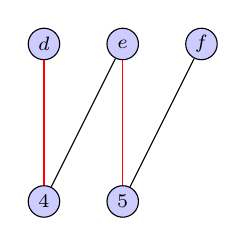
\begin{tikzpicture}[scale=1, every node/.style={circle, draw, fill=blue!20, inner sep=1pt, font=\scriptsize, minimum size=4mm}]
            \node (d) at (3, 2) {\(d\)};
            \node (e) at (4, 2) {\(e\)};
            \node (f) at (5, 2) {\(f\)};

            \node (4) at (3, 0) {\(4\)};
            \node (5) at (4, 0) {\(5\)};

            \draw[red] (d) -- (4);
            
            \draw (e) -- (4);
            \draw[red] (e) -- (5);
            
            \draw (f) -- (5);
        \end{tikzpicture}
    }
}
	\end{td-sol}
}{}


% ----- Consignes exo 10 ----- %
\begin{td-exo}[Convexité]\,\\ % 10 
	% fill
\end{td-exo}

% ----- Solutions exo 10 ----- %
\iftoggle{showsolutions}{
	\begin{td-sol}[]\,\\ %
		A remplir %TODO solve exercise 10
	\end{td-sol}
}{}


% ----- Consignes exo 11 ----- %
\begin{td-exo}[Convexité]\,\\ % 11 
	% fill
\end{td-exo}

% ----- Solutions exo 11 ----- %
\iftoggle{showsolutions}{
	\begin{td-sol}[]\,\\ %
		A remplir %TODO solve exercise 11
	\end{td-sol}
}{}


% ----- Consignes exo 12 ----- %
\begin{td-exo}[Convexité]\,\\ % 12 
	% fill
\end{td-exo}

% ----- Solutions exo 12 ----- %
\iftoggle{showsolutions}{
	\begin{td-sol}[]\,\\ %
		On part de \(m\) non saturé et on calcule un arbre 
		de couplage. Le sommet \(j\) est non saturé donc 
		on a le chemin augmentant \(mj\), on le rajoute au couplage.

		\vspace{0.5cm}
		% Figure 1
\ffigbox[\FBwidth]{
\caption{\centering Graphe \(G\)}\label{Fig:td_2_ex_12_a}
}{
    \fbox{
        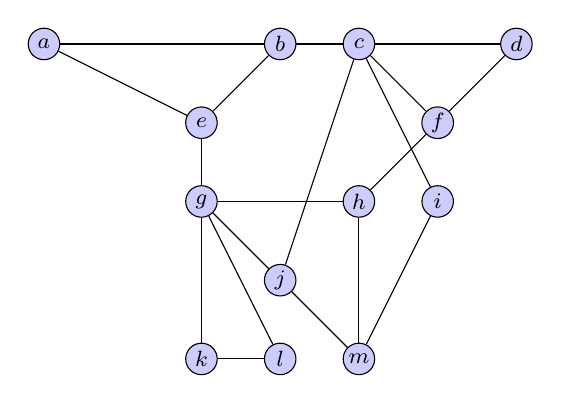
\begin{tikzpicture}[scale=1, every node/.style={circle, draw, fill=blue!20, inner sep=1pt, font=\footnotesize, minimum size=4mm}]
            \node (a) at (-2, 2) {\(a\)};
            \node (b) at (1, 2) {\(b\)};
            \node (c) at (2, 2) {\(c\)};
            \node (d) at (4, 2) {\(d\)};
            \node (e) at (0, 1) {\(e\)};
            \node (f) at (3, 1) {\(f\)};
            \node (g) at (0, 0) {\(g\)};
            \node (h) at (2, 0) {\(h\)};
            \node (i) at (3, 0) {\(i\)};
            \node (j) at (1, -1) {\(j\)};
            \node (k) at (0, -2) {\(k\)};
            \node (l) at (1, -2) {\(l\)};
            \node (m) at (2, -2) {\(m\)};


            \draw (a) -- (b);
            \draw (a) -- (e);

            \draw (b) -- (c);
            \draw (b) -- (e);
            
            \draw (e) -- (g);

            \draw (c) -- (j);
            \draw (c) -- (i);
            \draw (c) -- (f);
            \draw (c) -- (d);

            \draw (g) -- (k);
            \draw (g) -- (j);
            \draw (g) -- (h);
            \draw (g) -- (l);

            \draw (j) -- (m);
            
            \draw (i) -- (m);

            \draw (f) -- (h);
            \draw (f) -- (d);

            \draw (k) -- (l);

            \draw (h) -- (m);
        \end{tikzpicture}
    }
}

		On part de \(d\) non saturé.
		% d -- c
		% c -- f en rouge, c bleu, d et f rouges

		On trouve \(df\) une arête entre 2 sommets rouges,
		c'est-à-dire un blossom. On le contracte.
		% a -- b -- "cdf"

		On part de \(i\) non saturé et on trouve \(i-cdf\) un 
		chemin augmentant. En décontractant le blossom, 
		on trouve \(i-c-f-d\) un chemin augmentant.
		% insert another graph here

		On augmente \(M\), on a \(M\) final:
		\begin{equation*}
			M = \{ic, fd, ae, gh, jm, kl\}
		\end{equation*}
		seul \(b\) est non saturé: \(M\) est maximum
	\end{td-sol}
}{}


% ----- Consignes exo 13 ----- %
\begin{td-exo}[Convexité]\,\\ % 13 
	% fill
\end{td-exo}

% ----- Solutions exo 13 ----- %
\iftoggle{showsolutions}{
	\begin{td-sol}[]\,\\ %
		A remplir %TODO solve exercise 13
	\end{td-sol}
}{}


% ----- Consignes exo 14 ----- %
\begin{td-exo}[Convexité]\,\\ % 14 
	% fill
\end{td-exo}

% ----- Solutions exo 14 ----- %
\iftoggle{showsolutions}{
	\begin{td-sol}[]\,\\ %
		A remplir %TODO solve exercise 14
	\end{td-sol}
}{}

%%%%%%%%%%%%%%%%%%
% ce qu'on a vu en cours:
% - corollaire 1 de hall
% - corollaire 2 de hall


    \newpage
    \section*{TD3 --- Satisfaction de contraintes}\label{sec:TD3}
    \addcontentsline{toc}{section}{\nameref{sec:TD3}}
    \setcounter{section}{3}
    \setcounter{tdcounter}{0}
    \begin{td-exo}[Le puzzle du zèbre]
    Le puzzle du zèbre est un jeu logique bien connu, atribué à Albert Einstein
    ou à Lewis Caroll, sans certitude que l'inventeur soit l'un des deux. Il
    existe plusieurs variantes de ce jeu, voici l'énoncé d'origine.
    
    % TODO inserer enonce ici

    Il faut aussi ajouter que les maisons sont supposées être sur une ligne. La
    question \og{}qui boit de l'eau\fg{} doit être comprise comme \og{}sachant que
    quelqu'un boit de leau, qui est-ce?\fg{} (sinon on peut trouver une solution
    où personne ne boit de l'eau). De même la question \og{}qui possède le zèbre\fg{} 
    doit être comprise comme \og{}sachant que quelqu'un possède le zèbre, qui est-ce?\fg{}.
    Si on sait que quelqu'un boit de l'eau et que quelqu'un possède un zèbre, on peut 
    en fait déterminer qui vit où, la couleur de sa maison, sa nationalité, ce qu'il 
    boit et fume et son animal de compagnie.

    Modéliser ce problème comme un problème de satisfaction de contraintes.

    Quelle est la taille de l'espace de recherche?

    Peut-on reformuler certaines contraintes pour diminuer l'espace de recherche?
\end{td-exo}

    \newpage
    \section*{TD4 --- Résolution de CSP}\label{sec:TD4}
    \addcontentsline{toc}{section}{\nameref{sec:TD4}}
    \setcounter{section}{4}
    \setcounter{tdcounter}{0}
    \section{Modélisation}\label{sec:s_4}
% ----- Consignes exo 30 ----- %
\begin{td-exo}[Propriétés liées à la mesure au pire cas]\, % 30 
	\begin{enumerate}
		\item Soit \(\Pi\) un problème de maximisation appartenant à la classe \(\mathcal{NPO}\) ayant un ratio \(\delta\) pour la mesure.
		Montrer que cela implique que le ratio dans le pire cas est de \(\delta\).

		\item Sur le problème du \textsc{TSP}, considérons une instance \(I = (K_n, \overset{\rightarrow}d)\) avec \(\overset{\rightarrow}d\) le vecteur des arêtes-distances.
		Alors, pour n'importe quelle transformation affine
		\begin{equation*}
			\overset{\rightarrow}d \coloneqq \gamma \cdot \overset{\rightarrow}d + \mu \cdot \overset{\rightarrow}1
		\end{equation*}
		avec \(\gamma,\mu \in \bb Q\) produit une approximation différentielle équivalente à celle obtenue pour \(I\).
	\end{enumerate}
\end{td-exo}

% ----- Solutions exo 30 ----- %
\iftoggle{showsolutions}{ 
	\begin{td-sol}[]\ % 30
		
	\end{td-sol}
}{}


% ----- Consignes exo 31 ----- %
\begin{td-exo}[Mesure différentielle: borne inférieure pour le problème du \textsc{Bin Packing}]\,\\ % 31 
	Montrer que \textsc{Bin Packing} ne peut être résolu par un algorithme polynomial à rapport différentiel minoré par \(\frac{n-1}{n}\).

	Pour cela, on pourra supposer l'existence d'un tel algorithme et arriver à une contradiction.
\end{td-exo}

% ----- Solutions exo 31 ----- %
\iftoggle{showsolutions}{ 
	\begin{td-sol}[]\ % 31
		On suppose qu'il existe un algorithme polynomial \(A\) pour \textsc{Bin Packing} tel que 
		\begin{equation*}
			\frac{n - A(I)}{n - \textsc{opt}(I)} \geq \frac{n-1}{n}
		\end{equation*}
		alors
		\begin{equation*}
			A(I) - \textsc{opt}(I) \leq 1 - \frac{\textsc{opt}(I)}{n} < 1
		\end{equation*}
		or \(A(I)\) et \(\textsc{opt}(I)\) sont des entiers, donc \(A(I) = \textsc{opt}(I)\) et \(A\) est un algorithme polynomial pour \textsc{Bin Packing}, ce qui est impossible.
	\end{td-sol}
}{}


% ----- Consignes exo 32 ----- %
\begin{td-exo}[title]\,\\ % 32 
	
\end{td-exo}

% ----- Solutions exo 32 ----- %
\iftoggle{showsolutions}{ 
	\begin{td-sol}[]\ % 32
		
	\end{td-sol}
}{}


% ----- Consignes exo 33 ----- %
\begin{td-exo}[title]\, % 33 
	
\end{td-exo}

% ----- Solutions exo 33 ----- %
\iftoggle{showsolutions}{ 
	\begin{td-sol}[]\ % 33
		
	\end{td-sol}
}{}


% ----- Consignes exo 34 ----- %
\begin{td-exo}[Sur le problème du voyageur de commerce]\,\\ % 34 
	Le problème du voyageur de commerce consiste à effectuer un circuit Hamiltonien de cout minimum dans un graphe complet non orienté.
	Pour cela nous considérons \(n+1\) villes tel que le cout entre deux villes est donné par la matrice \(C = (c_{ij})\) où \(c_{ij}\) est le cout pour aller de la ville \(i\) à la ville \(j\).
	\begin{enumerate}
		\item Pourquoi le problème du voyageur de commerce est étudié dans le cadre d'un graphe complet valué et non dans un graphe quelconque?
		\item Rappeler la définition d'un circuit Hamiltonien.
		Quelles conséquences sur les degrés des sommets du circuit Hamiltonien?
		Modéliser ce problème par un programme linéaire en nombres entiers en justifiant les contraintes.
		\item Donner un exemple qui satisfait les contraintes du programme linéaire en nombres entiers mais qui n'est pas une solution réalisable du voyageur de commerce. 
		Quel est l'inconvénient des nouvelles contraintes? (Penser aux problèmes des sous-tours.)
		\item Nous ajoutons au programme linéaire en nombres entiers les contraintes suivantes:
		\begin{equation*}
			u_i - u_j + n x_{ij} \leq n-1, \quad \forall 1 \leq i \neq j \leq n
		\end{equation*}
		Montrer que les contraintes qu'on vient d'ajouter définissent bien le problème du voyageur de commerce.
		\item Comment appele-t-on ce type de programme linéaire?
	\end{enumerate}
\end{td-exo}

% ----- Solutions exo 34 ----- %
\iftoggle{showsolutions}{ 
	\begin{td-sol}[]\ % 34
		
	\end{td-sol}
}{}




% ----- Consignes exo 35 ----- %
\begin{td-exo}[Contraintes serrées et solutions] % 35
	On considère
	\begin{equation*}
		P = \begin{cases}
			\max z &= 6x_1 + 5x_2\\
			x_1 + x_2 &\leq 8\\
			-2x_1 + 3x_2 &\leq 6\\
			x_1 - x_2 &\leq 2\\
			x_1,x_2 &\geq 0.
		\end{cases},\quad
		D = \begin{cases}
			\min z = 8u_1 + 6u_2 + 2u_3\\
			u_1 - 2u_2 + u_3 &\geq 6\\
			u_1 + 3u_2 - u_3 &\geq 5\\
			u_i &\geq 0,\ i=1,2,3.
		\end{cases}
	\end{equation*}
	En supposant que la solution optimale du primal est \(x=(5,3)\), donner 
	la solution du dual. Quelles sont les contraintes serrées pour le primal et le dual.
\end{td-exo}

% ----- Solutions exo 35 ----- %
\iftoggle{showsolutions}{
	\begin{td-sol}[]\ % 35
		Supposons que la solution optimale du primal est \(x=(5,3)\). Les contraintes donnent alors:
		\begin{equation*}
			\begin{aligned}
				5 + 3 \leq 8 &\iff 8 \leq 8\\
				-2\cdot 5 + 3\cdot 3 \leq 6 &\iff -1 \leq 6\\
				5-3 \leq 2 &\iff 2 \leq 2
			\end{aligned}
		\end{equation*}
		Les contraintes 1 et 3 sont serrées, la contrainte 2 ne l'est pas. Donc on sait que 
		\begin{equation*}
			u_1 > 0,\ u_2 = 0,\ u_3 > 0.
		\end{equation*}
		En rentrant cela dans le dual on obtient:
		\begin{equation*}
			\begin{cases}
				u_1 + u_3 \geq 6\\
				u_1 - u_3 \geq 5\\
			\end{cases}
		\end{equation*}
		Alors, la solution optimale est \((u_1 = \frac{11}2, u_2 = 0, u_3 = \frac12)\).
	\end{td-sol}
}{}






    % \newpage
    % \section*{TD3 --- Satisfaction de contraintes}\label{sec:TD3}
    % \addcontentsline{toc}{section}{\nameref{sec:TD3}}
    % \setcounter{section}{3}
    % \setcounter{tdcounter}{0}
    % \begin{td-exo}[Le puzzle du zèbre]
    Le puzzle du zèbre est un jeu logique bien connu, atribué à Albert Einstein
    ou à Lewis Caroll, sans certitude que l'inventeur soit l'un des deux. Il
    existe plusieurs variantes de ce jeu, voici l'énoncé d'origine.
    
    % TODO inserer enonce ici

    Il faut aussi ajouter que les maisons sont supposées être sur une ligne. La
    question \og{}qui boit de l'eau\fg{} doit être comprise comme \og{}sachant que
    quelqu'un boit de leau, qui est-ce?\fg{} (sinon on peut trouver une solution
    où personne ne boit de l'eau). De même la question \og{}qui possède le zèbre\fg{} 
    doit être comprise comme \og{}sachant que quelqu'un possède le zèbre, qui est-ce?\fg{}.
    Si on sait que quelqu'un boit de l'eau et que quelqu'un possède un zèbre, on peut 
    en fait déterminer qui vit où, la couleur de sa maison, sa nationalité, ce qu'il 
    boit et fume et son animal de compagnie.

    Modéliser ce problème comme un problème de satisfaction de contraintes.

    Quelle est la taille de l'espace de recherche?

    Peut-on reformuler certaines contraintes pour diminuer l'espace de recherche?
\end{td-exo}
\end{document}

